% uw-wkrpt-se.tex - An example work report that uses uw-wkrpt.cls
% Copyright (C) 2002,2003  Simon Law
% 
% This program is free software; you can redistribute it and/or modify
% it under the terms of the GNU General Public License as published by
% the Free Software Foundation; either version 2 of the License, or
% (at your option) any later version.
% 
% This program is distributed in the hope that it will be useful,
% but WITHOUT ANY WARRANTY; without even the implied warranty of
% MERCHANTABILITY or FITNESS FOR A PARTICULAR PURPOSE.  See the
% GNU General Public License for more details.
% 
% You should have received a copy of the GNU General Public License
% along with this program; if not, write to the Free Software
% Foundation, Inc., 59 Temple Place, Suite 330, Boston, MA  02111-1307  USA
%
%%%%%%%%%%%%%%%%%%%%%%%%%%%%%%%%%%%%%%%%%%%%%%%%%%%%%%%%%%%%%%%%%%%%%
%
% We begin by calling the workreport class which includes all the
% definitions for the macros we will use.
\documentclass[se]{uw-wkrpt}

% LaTeX preamble: load some packages to add functionality
\usepackage{graphicx} % Include graphic importing

\usepackage[T1]{fontenc} % Better fonts
\usepackage{ae,aecompl}

\usepackage{indentfirst} % Indent first paragraph of each section

\usepackage[titletoc,title]{appendix} % Prefix appendix letters with `Appendix'

\usepackage{amsmath}
%\usepackage{scrextend}
\usepackage{fullpage}
\usepackage{amssymb}
\usepackage{alltt}
\usepackage{tkz-graph}
\usepackage{parskip}
\usepackage{enumitem}
\usepackage{bytefield}
\usepackage{listings,color}
\usepackage{float}


% Use the algorithmicx package for pseudocode
\usepackage{algorithm}
\usepackage{algpseudocode}

% Use biblatex for references
\usepackage[style=ieee,sorting=none,dateabbrev=false,backend=biber]{biblatex}
\addbibresource{uw-wkrpt-bib.bib} % Specify the bibliography file

% This needs to be the last package loaded
\usepackage[pdftex]{hyperref} % Generate PDF links and bookmarks.
\hypersetup{
  bookmarks=true,
  bookmarksnumbered=true
}

\definecolor{verbgray}{gray}{0.9}

\lstnewenvironment{code}{%
  \lstset{backgroundcolor=\color{verbgray},
  frame=single,
  framerule=0pt,
  basicstyle=\ttfamily,
  columns=fullflexible}}{}

% http://www.martin-demling.de/2011/06/memory-maps-in-latex-using-the-bytefield-package/
\newcommand{\memsection}[4]{
	\bytefieldsetup{bitheight=#3\baselineskip} % define the height of the memsection
	\bitbox[]{10}{
		\texttt{#1} % print end address
		\\ \vspace{#3\baselineskip} \vspace{-2\baselineskip} \vspace{-#3pt} % do some spacing
		\texttt{#2} % print start address
	}
	\bitbox{16}{#4} % print box with caption
}


% Now we will begin writing the document.
\begin{document}

%%%%%%%%%%%%%%%%%%%%%%%%%%%%%%%%%%%%%%%%%%%%%%%%%%%%%%%%%%%%%%%%%%%%%
%% IMPORTANT INFORMATION
%%%%%%%%%%%%%%%%%%%%%%%%%%%%%%%%%%%%%%%%%%%%%%%%%%%%%%%%%%%%%%%%%%%%%

%% First we, should create a title page.  This is done below:
% Fill in the title of your report.
\title{OS WOW RTX Design Documentation}

% Fill in your name.
\author{Fasih Awan, Joshua Kalpin, Si Chuang Li, John Zanutto}

% Fill in your student ID number.
\uwid{20414848, 20414492, 20413578, 20418726}

% Fill in the name of the PNG file with your signature, or leave unchanged.
\signature{signature}

% Fill in your home address.
\address{123 University Ave. W.\\*
         Waterloo, ON\ \ N2L 3G1}

% Fill in your employer's name.
\employer{SE 350}

% Fill in your employer's city and province.
\employeraddress{Thomas Reidemeister}

% Fill in your school's name.
\school{University of Waterloo}

% Fill in your faculty name.
\faculty{Software Engineering}

% Fill in your student user ID
\userid{fawan, jkalpin, sc6li, jzanutto}

% Fill in your e-mail address.
\email{jrhacker@engmail}

% Fill in your term.
\term{3A}

% Fill in your program.
\program{Software Engineering}

% Fill in the department chair's name.
\chair{Dr.\ A.\ Morton}

% Fill in the department chair's mailing address.
\chairaddress{Software Engineering\\*
              University of Waterloo\\*
	      Waterloo, ON\ \ N2L 3G1}

% If you are writing an "SE-confidential" report, uncomment the next line.
%\confidential{SE-confidential}

% If you want to specify the date, fill it in here.  If you comment out
% this line, today's date will be substituted.
%\date{April 24, 2012}

% Now, we ask LaTeX to generate the title.
\maketitle

%%%%%%%%%%%%%%%%%%%%%%%%%%%%%%%%%%%%%%%%%%%%%%%%%%%%%%%%%%%%%%%%%%%%%
%% FRONT MATTER
%%%%%%%%%%%%%%%%%%%%%%%%%%%%%%%%%%%%%%%%%%%%%%%%%%%%%%%%%%%%%%%%%%%%%
%% \frontmatter will make the \section commands ignore their numbering,
%% it will also use roman page numbers.
\frontmatter

% Next, we need to make a Table of Contents, List of Figures and 
% List of Tables.  You will most likely need to run LaTeX twice to
% get these correct.  The first pass for LaTeX to figure out the
% labels, and the second pass to put in the right references.

\setcounter{tocdepth}{1}

\tableofcontents

%%%%%%%%%%%%%%%%%%%%%%%%%%%%%%%%%%%%%%%%%%%%%%%%%%%%%%%%%%%%%%%%%%%%%
%% REPORT BODY
%%%%%%%%%%%%%%%%%%%%%%%%%%%%%%%%%%%%%%%%%%%%%%%%%%%%%%%%%%%%%%%%%%%%%
%% \main will make the \section commands numbered again,
%% it will also use arabic page numbers.
\mainmatter

% You must have an Introduction
\section{Introduction}\label{sec:intro}

\subsection{About}

This report is a detailed design document describing the OS WOW Real-Time Operation System designed by Fasih Awan, Joshua Kalpin, Si Chuang Li and John Zanutto. This operating system was implemented for the Keil MCB1700 board populated with an NXP LPC1768 microcontroller. 

This operating system was created over the span of three months during the creators' 3A term in Software Engineering. It was developed in four parts adding more features each time. The first part involved creating basic memory management and a multiprogramming environment. The second part added the challenge of interrupt driven I/O, timer interrupts and inter-process communication. The third part added more user processes. Lastly, the fourth part of the project included timing tests and this report.

\subsection{Purpose}

The purpose of this report is to provide the reader with detailed documentation on the OS WOW operating system. This includes the following information:  First, this report will document the APIs that are available to users of the operation system. Second, details on how interrupts are handled within the operating system will be specified. Third, the various system, user and test processes will be explained. Fourth, details on how the operating system is initialized, including memory and processes will be provided. Fifth, there will be details on testing, design challenges and timing analysis on the functions of the operating system. Lastly, the data structures and global variables that the kernel uses.

\section{Kernel API} \label{sec:kernel}

\subsection{Memory}

A memory block is a piece of memory that the user can dynamically request from the kernel to use such as for an array or other complex data structure. Internally, a memory block is represented as a doubly-linked-list node with some extra headers for message passing. Refer to Figure~\ref{fig:memory-block} in the Initialization section for more information about how these blocks are initialized.

The kernel keeps track of the available memory with a global pointer \texttt{free\_mem} that points to the first block of the list of free memory blocks. Whenever a memory block is requested, the front of this list is removed (if the list is not empty) and is given to the requester. Whenever a memory block is released, the given block is added to the front of this list.

\subsubsection{Request Memory}
\begin{code}
void* request_memory_block()
\end{code}

This method takes zero arguments and returns an address to a piece of memory that the caller can use. The returned address points to a continuous block of memory of size \texttt{0x1E4} bytes that the current process can read and write to. Currently, the memory protection unit is disabled so if the process reads or writes outside of \texttt{returned address + 0x1E4}, then undefined behaviour will occur.

If the system is out of memory, then the calling process will be pre-empted and will be placed on its priority's memory blocked queue until more memory becomes available (i.e. when another process releases their memory). It is recommended that once the user is finished with their allocated block that they release it otherwise the system will run out of memory very quickly.

\subsubsection{Release Memory}
\label{sec:release-memory-block}
\begin{code}
int32_t release_memory_block(void*)
\end{code}

This method takes in a pointer returned by \texttt{request\_memory\_block()}, deallocates it, and returns 0 if successful. If there was an error or if the pointer was invalid such as NULL or out of the range of the RAM, this method returns -1. This method also checks if there are currently any processes blocked on memory with a priority greater than or equal to the calling process. If so, then the current process will get pre-empted and the scheduler will get called instead of continuing with the current process.

\subsubsection{Example Usage of Requesting and Releasing Memory}
\begin{code}
#include "memory.h"
void example_process(void) {
    int* array;
    while (1) {
        array = (int*) request_memory_block();
        array[0] = 0xDEADC0DE;
        release_memory_block(array);
    }
}
\end{code}

\subsection{Process Management}

\subsubsection{Process Control Block}

A Process Control Block (PCB) specifies the various pieces of information that a process needs to be scheduled and executed. A PCB contains the process' id, current state, priority, top of stack pointer and a message queue for receiving messages.

\begin{code}
//The PCB
typedef struct {
    uint32_t pid; //process id
    PROCESS_STATE state; //current state
    uint32_t priority; //process priority
    uint32_t* stack_ptr; //top of stack
    linkedlist_t msg_queue; //message queue
} pcb_t;
\end{code}

Processes can have one of five valid priority levels from 0 (\texttt{HIGHEST}) to 4 (\texttt{LOWEST}). The lowest priority level is reserved for the Null Process. All other priority levels can be used by any process.

Processes can be in one of five states. Before a process is first run, it is in the \texttt{NEW} state. When a process is run it enters the \texttt{RUNNING} state. Once a process finishes or is pre-empted and is not blocked, it enters the \texttt{READY} state. If a process is either blocked on receiving a message or memory it either enters into the \texttt{MSG\_BLOCKED} or \texttt{MEM\_BLOCKED} state depending on what is it blocked on. When a process terminates it enters the \texttt{EXIT} state. However, no processes ever terminate in the operating system, so no processes will enter this state.

\subsubsection{Releasing the Processor}

\begin{code}
int32_t release_processor()
\end{code}

When a process has completed a task or is blocked it should release the processor to another process. This is done by calling \texttt{release\_processor()}, a function that takes no arguments and returns 0 on success. This function chooses the next process, saves the current process' state and switches to the next process.

To choose the next process and enqueue the current process, the operating system first checks if the current process is blocked or not. If it is blocked, it checks all possible priority levels for the next available process to queue. Otherwise, it only checks if there is a process on a ready queue with a higher or equal priority to schedule next. If there is no process that satisfies this condition, then the current process is chosen as the next process. Otherwise, the highest priority process at the front of its respective ready queue is chosen. After the next process is chosen, the current process is either put onto a ready queue or a blocked queue for its priority depending on its current state.

Once the next process is chosen, the context switch occurs. If we are not changing process' (i.e. the next process is the currently running one), the operating system skips this step. This operation occurs in two slightly different ways depending on if the operating system is switching to a new process or a process that has already ran.

In both cases, the operating system will save the current stack value to the old process' PCB. Next, it sets the current process to running and sets the stack pointer to the current PCB's stack pointer. Lastly, if the new process has never been run, the operating system switches from handler mode to user mode. Once the function returns, the new process is immediately invoked.

\subsubsection{Changing a Process' Priority}

\begin{code}
int32_t set_process_priority(int32_t process_id, int32_t new_priority)
\end{code}

A process may invoke the \texttt{set\_process\_priority} function if it wishes to change its or another process' priority. This function takes two parameters, \texttt{process\_id}, the id of the process that it wishes to change the priority of, and \texttt{new\_priority}, the new priority of the chosen process. This function will return 0 if a valid process and priority are specified; otherwise, it returns -1.

The function works slightly differently depending on whether the process priority being changed is the calling process or another process. If the calling process' priority is changed, it is immediately changed. If there is a process with a priority greater than or equal to the current process after the change, the process is pre-empted. 

Otherwise, if the process whose priority is being changed is not the current process, its priority is changed and then it is moved from its old priority queue (state dependant), to a queue with its new priority. If the new priority is greater than or equal to the current process' priority, the current process is pre-empted.

\subsubsection{Getting a Process' Priority}

\begin{code}
int32_t get_process_priority(int32_t process_id)
\end{code}

A process may check its or another process' priority by calling the \texttt{get\_process\_priority} function. This function takes a single parameter, the process id of the process to be queried. If this is a valid process id, that process' priority is returned. Otherwise, -1 is returned.

\subsection{Inter-Process Communcation} \label{sec:ipc}

Inter-Process Communication is managed by using a messaging passing system within the operating system. Messages are handled in two parts, kernel and user messages. User messages contain two properties, the message type and the message data itself. Kernel messages contain other information such as the sender of the message, the receiver of the message, a linked list node for storing the message and its expiry time.

\begin{code}
//A kernel message
typedef struct {
    node_t msg_node;
    uint32_t sender_pid;
    uint32_t receiver_pid;
    uint32_t expiry;
    
    //user message parameters
    uint32_t msg_type;
    char msg_data[1];
} message_t;
\end{code}

\subsubsection{Send Message}

\begin{code}
int32_t send_message(int32_t process_id, void* message_envelope)
\end{code}

The \texttt{send\_message} takes in two parameters, a process id and a message envelope and will return 0 on success. The process id must be a valid process inside of the operating system otherwise the function will return 1. The message envelope to be sent must be created by the calling process. First, the process must request a memory block and cast it to be of type \texttt{msg\_buf\_t}. Then, the process can specify a type and message data to be sent.

Once a process sends a message, the kernel will then convert the message to be a kernel message. This is done by subtracting a offset equal to the size of the kernel header from the struct to reveal the user hidden properties. After doing this, the message is initialized with the sender process id, receiver process id and its linked list node is instantiated. The message is then added to the receiving process' message queue. If the receiving process was blocked on messages, it will then be added to its appriorite ready queue. Additionally, if the receiving process is of equal or higher priority to the current process, the current process will be pre-empted.

\subsubsection{Receive Message}

\begin{code}
void* receive_message(int32_t* sender_id)
\end{code}

The receive message function takes in one parameter, a pointer to an integer and will return the received message. The integer pointer passed in will be used to store the the process id of the process that sent the message. 

Once a process wants to receive a message, its message queue is queried to see if there are any waiting messages. If there are no messages available, the process is marked as \texttt{MSG\_BLOCKED}, added to its appropriate message blocked queue and the processor is released. Once there is a message available, it is popped off the process' message queue. Then, if there was a non-null parameter passed in, it stores the process id of the sending process inside of that pointer. Lastly, the message is converted back into a user message and returned to the user.

\subsubsection{Delayed Send}

\begin{code}
int32_t delayed_send(int32_t process_id, void* message, int32_t delay)
\end{code}

The delayed send method works alongside the timer interrupts. To start off, delayed send needs its own message queue since it needs to hold on to messages until its time to send them. First of all, another parameter for the message struct has to be added so that each message has an expiry time. Then, to actually store these messages so that they're separate from the regular message queue, a new linked list object is created that held these messages. The linked list object is created when the timer is initialized since that is where all the messages will be sent out from.

Delayed send starts off with some sanity checks such as if the delay was a value of 0, then the message should be sent directly using \texttt{send\_message}. After the sanity check, the message is initialized with the sender process id, receiver process id and its linked list node is instantiated. After the message has been initialized, the time delay set to the message is the value of the current timer count [~\ref{g_timer_count} ] plus the delay passed. This way it's easier to decide if the expiry date has been met. After that is done, the message queue for delayed send is iterated upon to look for an expiry time for a message to be greater than the current message. If the time is greater, then the current message will be placed right before that. This is basically using insertion sort. Once the message has been placed within the queue, the function exits. 

\subsubsection{Example Usage of Inter-Process Communication}

\begin{code}
#include "message.h"
#include "memory.h"

void some_process() {
	int32_t sender_id;
	msg_buf_t *msg = (msg_buf_t *)request_memory_block();
	
	msg.msg_type = DEFAULT;
	msg.msg_data[0] = 'D';
	send_message(PID_SOME_PROC, msg);
	msg = receive_message(&sender_id);
	
	if(sender_id == PID_SOME_PROC) {
		delayed_send(PID_SOME_PROC, msg, 1000);
	}
}
\end{code}

\section{Interrupts}\label{sec:interupt}

The operating system responds to interrupts from two places: UART-0 and an on-board timer. When an interrupt is received in the operating system, interrupts are immediately disabled to prevent nested interrupts from occurring.

\begin{code}
CPSID i ; disable interrupts
; save R4-R11, LR onto the stack
; handle interrupt by branching to the corresponding i-process
; load g_switch_flag into R4
CPSIE i ; enable interrupts
; if R4 == 1, branch to k_release_processor
; if R4 == 0, pop the top 12 words off the stack and write to R4-R11, PC
\end{code}

\subsection{Keyboard Interrupts} \label{sec:uart}

\subsubsection{UART I-Process}

The keyboard interrupt process takes an input on UART-0, processes it, and outputs it. Depending on the type of input, the system will respond differently (in the case of commands and hotkeys).

Keyboard interrupts are handled by the UART i-process. After disabling interrupts, the UART i-process is immediately invoked. The UART i-process reads input into a buffer and outputs each character as it is typed to the console allow the user to see their input. Once a carriage return (\texttt{$\backslash$r}) is received, buffer writing is postponed and the input will be processed. A special set of functions are invoked (post-fixed with \texttt{\_i} to allow this i-process to send messages without blocking or pre-emption. If it cannot obtain a memory block, the buffer is discarded. If it can obtain a memory block, the buffer is copied into a message envelope and sent to the KCD for decoding. 

This i-process will also check to see if it has any pending messages. This receive message call is non-blocking and will continue execution if no message is received. If a message is received, the message is printed using the UART output buffer. The i-process cannot be blocked because it is not scheduled regularly, so any regular system functions have modified versions designed to run specifically for the i-process.

\subsubsection{Debug Hotkeys}

Debugging hotkeys were designed to make debugging easier by outputting useful debug information when a key is pressed.. As such, they were designed to work without memory. A last check is performed in the keyboard i-process to determine if a hotkey is used. There are currently three implemented debug hotkeys. Each of these hotkeys produces a separate output in the UART-1 system console. These hotkeys will be enabled when the operating system is compiled with the \texttt{\_DEBUG\_HOTKEYS} flag enabled

The three hotkeys are as follows. If the "," key is pressed, the processes currently in the ready state are printed out. If the "/" key is pressed, processes that are messaged blocked are printed out. If the "." key is pressed, processes that are memory blocked are printed out.

\subsection{Timer Interrupts}

The timer interrupt is an interrupt that happens every millisecond. The interrupt handler first increments a global variable named \texttt{g\_timer\_count} which is just a timing variable. The interrupt handler then calls the timer interrupt process \texttt{timer\_i\_process}. 

The \texttt{timer\_i\_process} first gets the pointer to the front of its message queue, where delayed messages get sent, and then continues to check the front of the queue for any messages who have an expiry date that is less than the current timer count. If the expiry value for the message is less than the current timer count, then it is dispatched using \texttt{send\_message}. Once it hits a message at the front of the queue who's expiry date is greater than the current timer count, the process stops iterating the front of the queue and exits. Once the process exits, the interrupt handler enables interrupts, and exits.

\section{System and User Processes}\label{sec:proc}

\subsection{System Processes}

There are three system processes, the Null Process, the CRT Display, and the Keyboard Command Decoder.

\subsubsection{Null Process}

The Null Process runs as an infinite loop of releasing the processor. This process will only execute if all other processes are blocked, or there are no other processes in the system. As a result, this process has a special reserved priority that is the lowest possible in the system. Pseudocode for this process is below.

\begin{code}
while looping forever do
    release the processor
end
\end{code}

\subsubsection{Keyboard Command Decoder}

The Keyboard Command Decode (KCD) is designed to handle both the registration and the parsing of commands from the keyboard. The KCD takes all input in the form of a message from the UART i-process, determines which process corresponds to that command, and sends the command in a message to that process. The KCD will be message blocked upon first executing. The KCD parses input based on two types of messages, \texttt{DEFAULT} and \texttt{KCD\_REG}.

Default messages are treated as inputted commands, and are parsed by checking to see whether the command registered is contained in the contents of the message. If a command is found in the buffer (denoted by a \% symbol), it is checked against a list of registered commands. Commands are stored and implemented as an array of command structs (see below).
\begin{code}
typedef struct {
    uint32_t pid;
    char cmd[10];
} kcd_cmd_t;
\end{code}

When a command is discovered, it is compared against a command in the list of commands. The operating system assumes that all commands will be at most ten characters, and there will be no more than ten commands registered at any given time. The buffer is then copied into a new message envelope and sent to the process that registered the matching command via the process ID.

KCD registration messages are registered into the command list, along with the sender of the message and the type of command. The message is then released here. Registration with the KCD is done by sending a message of type \texttt{KCD\_REG} to the process with the specific command as the message data. This is then stored into the command list for future use and the memory allocated for the message is released.


\subsubsection{CRT Display}

The CRT Display process is a controller that provides a level of abstraction between the interrupt process and any user process trying to output. This mainly applies to processes that accept command input, such as the wall clock and the priority change process. 

The CRT receives a message and checks if it is of type \texttt{CRT\_DISPLAY}. If it is a valid message, it sends the message to the UART i-process (Section~\ref{sec:uart}) and triggers a keyboard interrupt to check for messages and perform the print operation. Otherwise, it will release the memory block.

\subsection{User Processes}

These processes can be found inside of \texttt{user\_proc.c}. These processes require registration of commands with the KCD, and only function on user input.

\subsubsection{Wall Clock}

The wall clock displays the time specified by the user in the HH:MM:SS format (hours, minutes, seconds). The user can set the time themselves, let the clock run from 00:00:00 upwards or terminate the clock.

The wall clock process first registers \texttt{\%W} command with the KCD. It then attempts to receive a message. The wall clock uses a state variable to determine whether the clock is currently running.

If the clock is running and the message received was sent by the clock itself, \texttt{delayed\_send} is used to send another message, with a 1 second delay, to itself. The message sent by \texttt{delayed\_send} is of the \texttt{DEFAULT} message type. The process then requests another memory block and sends a message of type \texttt{CRT\_DISPLAY} to the CRT containing the updated time.

If the clock is not running, or the message was not sent by the clock, it is validated against the registered command. If the command is valid, it is parsed for the correct information.

The \texttt{\%WR} command resets the clock. Specifically, it will set the current time to be zero, and begin running the clock. If the clock is just starting, a \texttt{CRT\_DISPLAY} message is sent to the CRT immediately to display the initial time 00:00:00. The process then proceeds to send delayed messages to itself. An error will be thrown if the input provided is not exactly \texttt{\%WR}.

The clock set command, \texttt{\%WS},  requires significant validation for the input. The colon locations, the spaces and all of the values are verified to determine whether the input is correct. The input is valid if it adheres to the following format:
\begin{code}
%WS HH:MM:SS
\end{code}

\texttt{H} represents hours, \texttt{M} represents minutes and \texttt{S} represents seconds. Each of these is required to be specified as two digits (e.g. 01:01:01). If the input matches this format, the clock is updated with the correct time, and a \texttt{CRT\_DISPLAY} message is sent to the CRT to display the new time immediately. The clock is then set to running if it is not currently running, and will begin sending delayed messages to itself.

The \texttt{\%WT} command terminates the clock if it is currently running. Otherwise, nothing happens. An error will be thrown if the input is not exactly \texttt{\%WT}.

Additionally, when the clock outputs, the output is sent to the top right corner of the terminal. This was done with by using special parsing modifiers in the output string. This can be seen below.
\begin{code}
"\033[s\033[1;69H\%02d:\%02d:\%02d\n\033[u"
\end{code}


\subsubsection{Change Process Priority}

The change priority process takes a user input command and sets the priority of a specified process to a specified priority when both are valid input. This process functions with the below input into the console by the user.

\begin{code}
%C [Process ID] [New Priority]
\end{code}

\texttt{Process ID} is the id of the process that will be changed, and ranges from process id 1 to process id 13. This id range excludes the i-processes and the Null Process because they have fixed priorities.

\texttt{New Priority} is the priority that the process will receive. This excludes priority 4 (denoted LOWEST in the priority enumerable) as that priority is reserved for the Null Process.

The change priority process first registers the \texttt{\%C} command with the KCD. It then will wait until it receives a message from the KCD.

The process does several error checks for validation. These include checking for invalid priorities, invalid process ids, process ids that are not numbers and priorities that are not numbers. Checking for valid command format is also done here (i.e. if spaces are used correctly). If the input is invalid, an error message is sent to the CRT for display. Otherwise, the \texttt{set\_process\_priority} method is called with the parsed process id and new priority. This process also outputs all input information to the debug window.

\subsubsection{Stress Test A}

The first stress test user process starts off by creating a new message and sending it to the KCD. The message itself is the string text \texttt{\%Z}, which is a command accepted by the KCD. After the message has been send, the process goes on a continuous loop where it calls \texttt{receive\_message}, which will block the process until it receives the message being sent to it. After the message has been received, the process exits the continuous loop, and enters another loop.

The second loop first calls \texttt{request\_memory\_block} to allocate memory for the message envelope. After receiving memory, it prepares the message block by assigning the message type to be \texttt{COUNT\_REPORT} which will allow the target process to continue its tasks. The sender of the message is set to the second user stress test process.


\subsubsection{Stress Test B}

This stress test process runs in a continuous loop and calls \texttt{receive\_message}. When it receives, this process immediately forwards that message to the third stress test process, process C.


\subsubsection{Stress Test C}

This process receives the messages which were created and sent in stress test A and then relayed by stress test B. This process starts out by creating a circular buffer \texttt{message\_queue} which acts as a message queue. The message queue will hold all the messages that this process receives.

Once the message queue has been initialized, the process enters a loop. First it checks if the message queue is empty, and if it is then the process calls \texttt{receive\_message} and remains blocked while waiting for a message to be sent to it. If the message queue was not empty, then a message is popped off from the front of the queue.

The process now checks the message type that it either received or popped off from the queue. In stress test A the message type was set to \texttt{COUNT\_REPORT}, which is what this process will now check for. If the message type is not \texttt{COUNT\_REPORT} then the process releases the memory block allocated, and then calls \texttt{release\_processor}. Then it reiterates from the beginning.

If the message type is \texttt{COUNT\_REPORT}, then the process checks if the value contained in the message is divisible by 20. If not, it releases the memory block for the message envelope, releases the process, and then reiterates. If the value is in fact divisible by 20, the process sends the message received to the CRT Display. Once sent, it creates a new message with a message type of \texttt{WAKEUP10} and sends it to itself using a delayed send with a delay of 10 seconds. The process now waits for that delayed message. While it waits it will queue up any messages that it receives in its own message queue, and when it finally receives that delayed message, it exits the loop and starts from the beginning again. 

\section{Test Processes}\label{sec:testproc}

Overall there are 6 test processes. The first five test processes test the functionality of the OS, and the sixth test polls all the results. In order to do that, an array of integers is defined which is used to set the result of the test as a $1$ or a $0$. All the test processes start off with a process priority of \texttt{MEDIUM}, and the polling process starts off with a priority of \texttt{LOW}. 


\subsection{Process 1}

The first test process tests the delayed send functionality. It creates a message with a specific text and sends it to itself with a delay of 1 \texttt{CLOCK\_INTERVAL} which is defined as $1000$ milliseconds. Then it calls \texttt{receive\_message} and blocks itself until it receives the message. The process then checks if the message text matches what was sent off using \texttt{strcmp}. It then sets its own priority to \texttt{LOW} and enters an infinite loop of calling \texttt{release\_processor}. 


\subsection{Process 2}

The second test process tests sending messages. It creates a new message with a specified string, and sends it to the third test process. The process then calls \texttt{receive\_message} and blocks itself until a message gets sent to it. Once the process receives its message, which the third process will be sending it, it compares the string text to make sure it matches the expected string, and then sets its own priority to \texttt{LOW}. It then enters an infinite loop of calling \texttt{release\_processor}. 


\subsection{Process 3}

The third test process also tests sending messages. It creates a new message with the string that the second test process is expecting, and then send it off using \texttt{send\_message}. It then calls \texttt{receive\_message} waiting for the message that was sent to it to come in. The process is blocked until then. Once it receives the message, it compares the string to the expected string, sets its own priority to \texttt{LOW} and then enters an infinite loop of calling \texttt{release\_processor}.


\subsection{Process 4 \& Process 5}

The fourth test process and the fifth test processes are similar processes. These processes test preemption based on process priority. They both have internal counters that are incremented. Both processes increment their counter every time the loop iterates twice. In the fourth test process when the counter hits 5, it sets the process priority of the fifth test process to \texttt{HIGH} and exits the first loop. It then checks if the fifth process finished first or not. In the fifth test process, when the counter hits 10 it sets the process priority of the fourth process to \texttt{HIGH}. The expected result is that the fourth process will finish first, and the fifth one finishes second. To check that, the process checks the numerical array created to see if the fifth test already completed. 


\subsection{Process 6}

The last test process just polls the result from the numerical arrays to see if they passed or failed, and then just outputs the results as $x/5\ \text{PASSED}$ and $y/5\ \text{FAILED}$. If any of the processes have not fully run yet, by checking if the test run array has a $0$ for their entry, then the process will run an infinite loop calling \texttt{release\_processor} until all other processes have ran. Once all of them have ran, it prints out the final results, and then goes into an infinite loop of calling \texttt{release\_processor}.

\section{Initialization}\label{sec:init}

At the start of the OS, the OS disables interrupts before it initializes the system, otherwise the interrupt handlers cannot run properly. Once everything is initialized properly, it re-enables interrupts and calls the scheduler to dispatch the first process.

\subsection{System APIs}
The first stage of the initialization is to setup the system APIs. First, the OS sets up the board and the system clock frequency. Second, \texttt{printf} is initialized for debugging. Third, UART0 is initialized to allow interrupt-driven I/O. Fourth, UART1 is initialized for program-driven I/O for debugging. Fifth, TIMER0 is initialized to send an interrupt every second. Sixth, TIMER1 is initialized to increment the \texttt{TC} every microsecond. Lastly, the LCD display is initialized to draw the OS's logo.

\subsection{Memory}

\begin{figure}[h]
\caption{Memory Map after Initialization}
\begin{bytefield}{}
    \begin{rightwordgroup}{User Memory Space}
    	\memsection{0x1000 7fff}{0x1000 6000}{4}{16 Process Stacks \\ (each size 0x200)} \\
    	\memsection{}{}{1.5}{-- unused --} \\
    	\memsection{}{}{3}{48 Memory Blocks \\ (each size 0x100)}
    \end{rightwordgroup} \\
    \memsection{0x100 aligned}{}{1.5}{-- unused --} \\
    \begin{rightwordgroup}{Kernel Memory Space}
        \memsection{}{}{1.5}{16 PCBs} \\
        \memsection{}{}{1.5}{16 PCB Nodes} \\
        \memsection{}{}{1.5}{5 Message Blocked Queues} \\
        \memsection{}{}{1.5}{5 Memory Blocked Queues} \\
        \memsection{}{}{1.5}{5 Ready Queues} 
    \end{rightwordgroup}\\
    \memsection{}{}{1.5}{-- 2 word(8 byte) guard --} \\
    \memsection{End of Image}{1000 0000}{3}{Process Image} \\
\end{bytefield}
 \label{fig:memory-map}
\end{figure}

After the system APIs have been initialized, the OS then defaults all of the memory from the end of the system image to the end of RAM with \texttt{0xDEADBEEF}. This makes it easier to debug because if a value after this stage is \texttt{0xDEADBEEF}, then it will be obvious that the value was not properly instantiated. Afterwards, the OS dynamically allocates memory for its data structures.  A map of the system memory after initialization is shown on Figure ~\ref{fig:memory-map}.

\subsubsection{Kernel Memory Space}

After the process image, the OS dynamically allocates space for all of its kernel's data structures. It first allocates 15 doubly-linked lists to represent 5 ready queues, 5 memory blocked queues, and 5 message blocked queues, one for each process priority. Unlike a traditional linked list implementation, the OS's linked lists do not dynamically allocate and free memory. Instead, the OS simply changes the node pointers because the kernel should never be blocked on memory or get pre-empted while it is running the scheduler. As a result, the OS's PCBs are wrapped with linked list nodes that are preallocated during its initialization stage. In total, the OS allocates 16 PCBs and 16 nodes structures for managing the PCBs.

\subsubsection{User Memory Space}
After the kernel's data structures have been instantiated, the OS then use the space above the PCBs for memory blocks. It first byte aligns the first memory block after the PCBs with \texttt{0x100}. This makes it easier to debug at the cost of at most \texttt{0xFF} memory. From the \texttt{0x100} byte-aligned address, the OS instantiates 48 new doubly linked blocks as shown below (i.e. each block has a pointer to its subsequently and previously instantiated blocks).

\begin{figure}[h] 
\caption{Memory Block}
\begin{bytefield}{}
    \memsection{0x200}{}{1.5}{\texttt{next}} \\
    \memsection{}{}{1.5}{\texttt{prev}} \\
    \begin{rightwordgroup}{Message Header}
    	\memsection{}{}{4}{-- 4 words (16 bytes) --}
    \end{rightwordgroup} \\
    \begin{rightwordgroup}{User space of size \texttt{0x1E4}}
    	\memsection{0x1E8}{0x4}{4}{\texttt{data}}
    \end{rightwordgroup} \\
    \memsection{}{}{1.5}{\texttt{padding = 0xABAD1DEA}} 
\end{bytefield}
\label{fig:memory-block}
\end{figure}

As shown in Figure~\ref{fig:memory-block}, each memory block is instantiated to be size \texttt{0x200}. However, the OS needs to reserve the top 6 words (24 bytes) for memory and message management (See Section~\ref{sec:ipc} for more information about messages). In addition, the OS reserves the bottom word (4 bytes) as a safety padding to help with debugging. This padding is required because it can detect if a user process writes past their allowable region by verifying the values in the padding. 

Finally, after all of these blocks are initialized, the OS sets the global \texttt{free\_mem} variable to point to the first memory block of this list. 

\subsection{Processes}
After both the kernel and user memory space have been initialized, the OS then moves on to initializing its PCBs with their corresponding process information. First the OS calls the processes' provided initialization methods, e.g. \texttt{set\_test\_procs()}, to fill in the OS's global process tables, e.g. \texttt{g\_test\_procs}. Each entry of the completed process table contains the corresponding process's id, priority, and pointer to where the process actually resides in memory. 

After the process tables are filled, the OS then iterates over all the processes in the process tables and initializes its PCBs in a number of steps. First, the \texttt{pid} and \texttt{priority} values are copied into the PCB. Second, the PCB state is set to \texttt{NEW}. Third, the PCB's message queue is initialized to be an empty linked list. Fourth, it initializes the process's stack (see Section~\ref{sec:setting-up-stack}). Lastly, it sets \texttt{stack\_ptr} to the appropriate location.
	
Although the i-processes do not need a stack because they rely on the kernel's stack whenever they run, it makes initialization simpler because the loop does not need to check process types. In addition, it is also of no consequence because there is still leftover space between the stacks and memory blocks.

\subsubsection{Setting up the Stack} \label{sec:setting-up-stack}

As specified in the board's documentation, to go from handler mode to thread mode, the OS uses the \texttt{BL 0xFFFF FFF9} instruction. This special instruction pops values off the stack frame, as shown in Figure~\ref{fig:stack-after-branch}, and copies them into their corresponding registers.
	
\begin{figure}
\caption{Stack after calling \texttt{BL 0xFFFF FFF9}}
\begin{bytefield}[rightcurly=.]{}
	\begin{rightwordgroup}{$\leftarrow$ SP is here after resuming to thread mode}
		\memsection{}{}{1.5}{-- NULL --} 
	\end{rightwordgroup} \\
	\memsection{}{}{1.5}{xPSR = \texttt{0x1000 0000}} \\
	\memsection{}{}{1.5}{PC = \texttt{proc\_start}} \\
    \memsection{}{}{1.5}{LR = \texttt{0x0}} \\
    \memsection{}{}{1.5}{R12 = \texttt{0x0}} \\
    \memsection{}{}{1.5}{R3 = \texttt{0x0}} \\
    \memsection{}{}{1.5}{R2 = \texttt{0x0}} \\
    \memsection{}{}{1.5}{R1 = \texttt{0x0}} \\
	\begin{rightwordgroup}{$\leftarrow$ SP initially points here in handler mode}
		\memsection{}{}{1.5}{R0 = \texttt{0x0}}
	\end{rightwordgroup} \\
\end{bytefield}
\label{fig:stack-after-branch}
\end{figure}
	
Normally, these values are automatically set when the user makes a system call from thread mode. However because the OS starts in handler mode, these values will not be on the stack when it tries to switch to thread mode the first time. In other words, the OS needs to write the default values onto the stack, as shown in Figure~\ref{fig:stack-after-branch}, and sets the \texttt{stack\_ptr} to point 8 words below the start of the stack so that the scheduler doesn't hard-fault.

\section{Testing}\label{sec:test}

\subsection{Verification}
To verify all the different features that were put into the Operating System, there were various ways that they were tested. Firstly, the test processes that were written for each deliverable focused solely on the different new features being added in. Mainly these test processes just verified that the functionality of anything that was implemented was fully working. These tests didn't include many edge cases, but just barebone functionality testing. The test processes would sometimes introduce small bugs that went unnoticed until the features written ran through the test processes. 

To actually test edge cases, most of the time it was done through input of different edge cases into the console. This usually meant several bad input strings were fed to the OS to see how it reacts to them. These usually found several edge cases that weren't previously considered. 

There was a specific case that required unit testing. To actually write the functionality of the string library in the OS, thorough unit testing was done in order to verify that all the string methods worked. Since it was easier to test these string methods outside of the OS itself, these unit tests were done externally, and were not including in the OS itself.

\subsection{Debugging}

To actually fix any bugs encountered, the debugging tool that was a part of the Keil IDE was used heavily. This involved tracking several local variables to see how they changed as certain functions were called, and using breakpoints and going step by step through the code to see where it might have been faulting or resulting in a bug. The memory watch was used to see how the bits in the memory of the OS changed to see if any discrepancy occurred. Along with using breakpoints and watch windows, debug flags were set to output debug print statements that were defined, in order to see if the code ever hit that section of the method, and if the variable that was being output was just garbage memory or not.

\section{Major Design Challenges}\label{sec:design}

\subsection{Mistakes}

There were a number of mistakes made in the course of developing OS WOW.

In Part 1, the linked list data structures in the operating system requested memory from the heap. This was a major problem because the kernel was using up a significant portion of the heap in the operating system. Additionally, there were strange pre-emption and scheduling issues that occured as a result. As a result, a lot of time was spent rewriting these in the second part of the project.

Another issue that occured was that the scheduler was giving priority to processes that were blocked on memory over other processes. This made the scheduler not use a First-In-First-Out (FIFO) approach when choosing the next process. Additionally, the operating system was not pre-empting processes when their priority was equal to the current process. This caused out of order execution in some test cases.

For the second part of the project, a number of different mistakes were found. First, the wall clock was not working as a 24-hour clock and instead was working on an 100 hour rollover. Second, there were a number of error cases not being checked for when the user sent messages to the wall clock process. Third, the wall clock was not being initialized properly and as a result hard faulted the test cases for this section of the project. Lastly, another strange bug that appeared was in the KCD. The KCD was not releasing memory blocks in some instances and a result blocking on memory was not acting as expected. A memory table was implemented but was removed because of the level of complexity it would have added in part two on top of the fact that it was not needed.

\subsection{Stumbling Blocks}

There were a number of stumbling blocks encountered in implementing OS WOW. First, trying to understand how to implement memory and various internal memory related data structures without a heap took a lot of time to figure out. Second, the Keil IDE was the source of much misery. The debugger would consistently crash without any reason when debugging hard faults. Additionally, there would be a vague algorithm error that would block downloading code onto the board. This significantly slowed down develop speed as a lot of time was wasted trying to figure out how to fix this problem. 

Another major stumbling block that was encountered was related to group dynamics. There was a lot of bickering and arguing over many aspects of the project. This lead to a lot of frustration and sometimes malice between the group members. These issues mainly centered around how much of a priority the project was, when to work on it, division of labour and various implementation details. Another potential factor contributing to this is that all of the group mates lived together and potentially spent way too much time together.

\subsection{Things To Change and Design Issues}

There would be a number of things that would be changed if OS WOW was built over again. First, a number of the data structures that were allocated at runtime (process queues, pcbs, pcb nodes, etc.) should have been allocated at compile time. This would have simplified the memory initialization process greatly and reduce overall code complexity. Second, the PCB nodes should have been part of the PCBs themselves, similar to how the messages functioned. This would have significantly reduced the operating system's memory usage and made keeping track of the location of PCBS much easier.

Another thing that would be changed is to have a better naming convention for global variables. Currently, global variables have an assortment of names that make them hard to identify and keep track of. The operating system should have followed a prefix convention, such as \texttt{g\_} for all global variables.

The last thing that would be changed would be to have some more consistency with return values. Currently a non-zero return value is considered a failure for a function call. However, more information on what the specific error is would have helped with debugging purposes.

\section{Timing Analysis}\label{sec:time}

To begin timing analysis, a different way to measure time was needed. Since the regular timer used for timer interrupts was only ever used to increment the timer count when an interrupt occurred, there was no way to measure timing since all the methods tested disabled interrupts. To remedy this situation, the timer was modified.

The new timer was instantiated just like the original timer, only now the MR0 register was left at 0 to avoid using interrupts. Instead, the internal clock was used, which was achieved by setting the TCR register to 1. Then to actually get the time value of the timer, a pointer reference was made to the TC register in the timer which holds the timer count. This reference was made global and used by the timing analysis process. 

The three methods tested: \texttt{request\_memory\_block}, \texttt{send\_message}, and \texttt{receive\_message}. 

Each method was tested 30 times to obtain a good amount of data. 
The following averages were calculated:
\begin{figure}
\begin{center}
\begin{tabular}{|c|c|}
\hline
Method & Average\\
\hline
Request Memory Block & 11.83 \\
\hline
Send Message & 12.03 \\
\hline
Receive Message & 11.09\\
\hline
\end{tabular}
\end{center}
\caption{Averages of all the methods tested}
\end{figure}

Figures ~\ref{fig:mem}, ~\ref{fig:send} and ~\ref{fig:receive} show the histograms for each method tested depicting the values obtained per method call recorded in $\mu s$.

\begin{figure}[bp!]
\centering
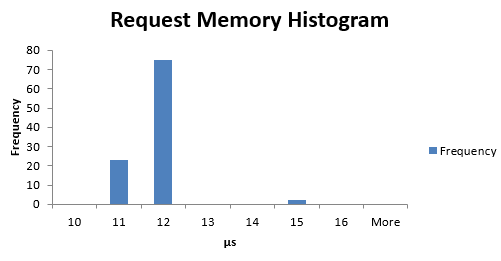
\includegraphics[width=120mm]{RequestMemoryHistogram.PNG}
\caption{Request Memory Times for Sample Size 30}
\label{fig:mem}
\end{figure}

\begin{figure}[bp!]
\centering
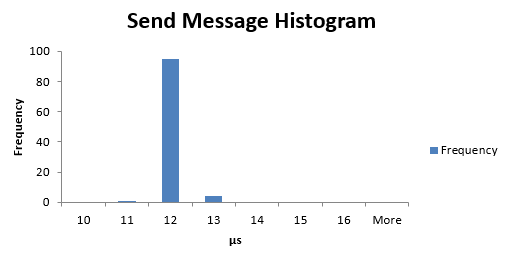
\includegraphics[width=120mm]{SendMessageHistogram.PNG}
\caption{Send Message Times for Sample Size 30}
\label{fig:send}
\end{figure}

\begin{figure}[bp!]
\centering
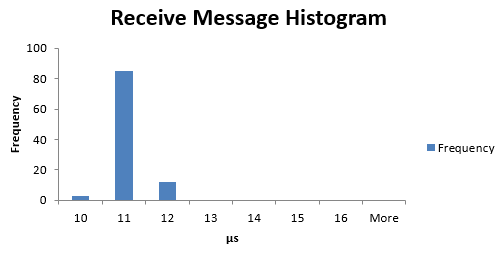
\includegraphics[width=120mm]{ReceiveMessageHistogram.PNG}
\caption{Receive Message Times for Sample Size 30}
\label{fig:receive}
\end{figure}

After analysing the OS structure, there were several things that may have affected the timing of the methods tested. Firstly, for \texttt{request\_memory\_block}, after the memory was obtained, it was completely zeroed out, which resulted in approximately $10\mu s$ of time in the recorded time. As for both \texttt{send\_message} and \texttt{receive\_message}, the main bottleneck there was the fact that after a message was received within the methods, it was sent off to a tracking function with stored the message within a buffer. This seemed to cause greatest delay for both of these functions. Figures ~\ref{fig:mem-nobottlenecks}, ~\ref{fig:send-nobottlenecks}, and ~\ref{fig:receive-nobottlenecks} show the new timings after bottlenecks are removed. 

Overall, the functioned resulted in a relatively consistent set of data points, showing that there was little to no discrepancy.

\begin{figure}[bp!]
\centering
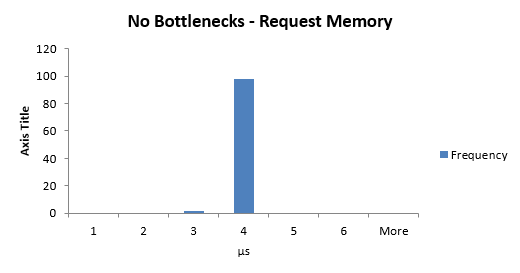
\includegraphics[width=110mm]{NB-RequestMemoryHistogram.png}
\caption{Request Memory Times for Sample Size 30 with Bottlenecks Removed}
\label{fig:mem-nobottlenecks}
\end{figure}

\begin{figure}[bp!]
\centering
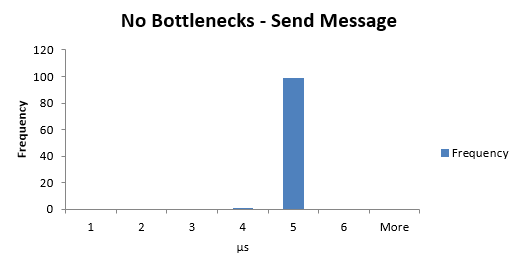
\includegraphics[width=110mm]{NB-SendMessageHistogram.png}
\caption{Send Message Times for Sample Size 30 with Bottlenecks Removed}
\label{fig:send-nobottlenecks}
\end{figure}

\begin{figure}[bp!]
\centering
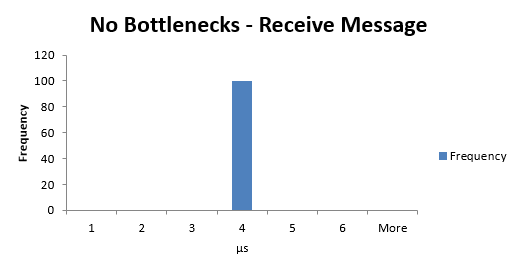
\includegraphics[width=110mm]{NB-ReceiveMessageHistogram.png}
\caption{Receive Message Times for Sample Size 30 with Bottlenecks Removed}
\label{fig:receive-nobottlenecks}
\end{figure}

\appendix
\begin{appendices}

\section{Global Variables}

\texttt{blocks\_allocated}: This variable represents the number of memory blocks that have been allocated from the heap. It is used to keep track of whether there was a memory block available to a process. This was then used to move it onto a ready queue from a blocked queue.

\texttt{pcb\_nodes}: This variable represents an array of linked list nodes for pcbs. These are indexed by their process ids and correspond to their respective PCBs. This was used to easily add and remove PCBs from their various queues.

\texttt{pcbs}: This variable represents an array of PCBs. These are indexed by their respective process ids. This is used to make querying other processes fast and efficient.

\texttt{current\_pcb\_node}: This variable represents the linked list node that holds the currently running process. This was created to make it easy to determine and/or modify the current process that is running.

\texttt{ready\_pqs}: This variable represents an array of 5 doubly linked lists that represent the ready priority queues for pcbs. This was exposed to make it simple to enqueue unblocked processes throughout the operating system.

\texttt{msg\_blocked\_pqs}: This variable represents an array of 5 doubly linked lists that represent the message blocked priority queues for pcbs. This was exposed to allow for the queue of blocked processes.

\texttt{mem\_blocked\_pqs}: This variable represents an array of 5 doubly linked lists that represent the memory blocked priority queues for pcbs. This was exposed to allow for the queue of blocked processes.

\texttt{g\_timer\_count} \label{g_timer_count}: This variable represents the current elapsed time for the interrupt timer in miliseconds. This is used to check whether to send a delayed message or not. This was exposed so that delayed send could record the time that a message was to be sent at.

\texttt{tc\_count}: This variable was used to perform our timing tests on our operating system. It is incremented every time the second timer ticks.

\end{appendices}

\end{document}
